\documentclass[UTF8,a4paper,11pt]{ctexart}

\usepackage{geometry}
\geometry{margin=2.5cm}

\usepackage{graphicx}
\usepackage{booktabs}
\usepackage{tabularx}
\usepackage{longtable}
\usepackage{array}
\usepackage{amsmath}
\usepackage{hyperref}
\usepackage{subcaption}
\usepackage{xcolor}
\usepackage{float}

\hypersetup{
  colorlinks=true,
  linkcolor=blue,
  citecolor=blue,
  urlcolor=blue
}

\DeclareRobustCommand{\feature}[1]{\texttt{\detokenize{#1}}}
\DeclareRobustCommand{\config}[1]{\texttt{\detokenize{#1}}}
\newcolumntype{Y}{>{\raggedright\arraybackslash}X}

\graphicspath{{figures/}}

\title{轴承剩余寿命、健康状态与早期故障检测的特征分析技术报告\\
\large A Feature Analysis Report for Bearing RUL, Health State, and Early Fault Detection}
\author{USTC/SSE BearingPrediction Project}
\date{\today}

\begin{document}

\maketitle
\tableofcontents
\newpage

\begin{abstract}
本文档整理轴承预测性维护项目中已完成的特征分析工作，覆盖 XJTU-SY 与 PHM2012 两个轴承 run-to-failure 数据集，以及剩余寿命（Remaining Useful Life, RUL）、健康状态（Health State）和早期故障检测（Early Fault Detection）三个任务。报告比较了 \config{manual_basic} 与 \config{manual_tsfresh_basic} 两类特征集，并基于已经归档的分析报告与推荐表给出最终技术结论\cite{feature_analysis_report,recommended_features,final_feature_decisions}。

核心结论是：当前下游 baseline 应使用 \config{manual_basic} 作为主线特征集。两个数据集上最稳定的特征族均为振幅/能量类时域特征，包括 magnitude、horizontal 与 vertical 通道上的均值、绝对均值、RMS、标准差和相关幅值统计。XJTU-SY 的 Early Fault 任务存在明显工况敏感性；PHM2012 则更一致地表现为 horizontal/magnitude 振幅特征主导。\config{manual_tsfresh_basic} 在 PHM2012 上可以运行，但 top \feature{tsfresh__} 特征主要重复 RMS、standard deviation、variance、maximum 等手工统计量；在 XJTU-SY 上 full-size tsfresh 被内存压力阻塞。因此，本阶段不采用 tsfresh 作为主线。

需要特别注意的是，\feature{mag__time__rms} 是实际健康指标（Health Indicator, HI）与首次预测时间（First Prediction Time, FPT）构造中的标签源特征（label-source feature）。它可以作为标签构造 sanity reference，但不能作为 Health State 或 Early Fault 的独立发现证据过度解释。
\end{abstract}

\section{引言}

轴承退化建模通常可以直接进入模型训练，但在本项目中，特征分析被放在 baseline 之前。原因有三点。

第一，RUL、Health State 和 Early Fault Detection 三个任务虽然都来自同一批振动快照，但它们对特征的需求并不完全相同。RUL 更强调随寿命推进的趋势性与相关性；Health State 更强调不同健康阶段的可分性；Early Fault Detection 更关注 FPT 前后是否出现可检测的早期差异。

第二，本项目的 Health State 与 Early Fault 标签由 HI/FPT 逻辑构造。若不先分析标签源特征与候选特征之间的关系，很容易把标签构造带来的高分误读为独立预测能力。因此，报告始终区分普通候选特征和 label-source reference。

第三，训练集之外的数据不能参与特征选择。本轮分析统一使用 \config{fit_scope=train_only}，即 ranking 只在训练集上拟合；验证集与测试集只用于分布检查和可视化审查。这一原则避免了把 test-bearing 信息泄漏进特征选择过程。

本文档不是新的实验报告，而是对已归档结果的技术整理。证据来自 \path{reports/feature_analysis/} 下的 Step F 至 Step L 报告、CSV 表格和精选图像，不引用本地临时 artifact run 目录。

\section{数据集与任务定义}

\subsection{XJTU-SY 数据与划分}

XJTU-SY 是轴承 run-to-failure 数据集。每个轴承在固定工况下从较健康状态运行到失效附近，原始数据以连续的振动快照组织；本项目的数据加载器把每个 \config{acc} 文件视为一个快照样本，并在索引中保留数据集、轴承、工况、样本序号与时间顺序。

本轮特征分析没有只依赖一个随机划分，而是使用三层检查：

\begin{itemize}[leftmargin=2em]
  \item 主划分 \config{xjtu_bearing_index_split}：同一工况下的前 3 个轴承进入训练集，第 4 个轴承进入验证集，第 5 个轴承进入测试集。这个划分用于回答“在覆盖三种工况的主训练设置下，哪些特征最有用”。
  \item 工况内 leave-one-bearing-out：分别在 35Hz12kN、37.5Hz11kN、40Hz10kN 内训练/验证/测试。这个划分用于回答“同一工况下，主结论是否稳定”。
  \item 跨工况划分 \config{xjtu_cross_condition}：训练集为 35Hz12kN，验证集为 37.5Hz11kN，测试集为 40Hz10kN。这个划分用于回答“特征排序是否只记住了某个工况的分布”。
\end{itemize}

三层检查是必要的。XJTU-SY 的工况差异会改变振动幅值、频谱位置和噪声水平；如果只看主划分，某些水平通道或频域特征可能看起来很强，但跨工况后会因为均值漂移或方差变化而降级。

\begin{table}[htbp]
\centering
\caption{XJTU-SY 分析划分}
\label{tab:xjtu_split_summary}
\scriptsize
\begin{tabularx}{\textwidth}{lYYYY}
\toprule
场景 & Train bearings & Val bearings & Test bearings & 用途 \\
\midrule
main & B1\_1--B1\_3; B2\_1--B2\_3; B3\_1--B3\_3 & B1\_4; B2\_4; B3\_4 & B1\_5; B2\_5; B3\_5 & 主三任务 ranking，7032/1679/505 samples。\\
C1 LOO & B1\_1--B1\_3 & B1\_4 & B1\_5 & 35Hz12kN 工况内稳定性，442/122/52 samples。\\
C2 LOO & B2\_1--B2\_3 & B2\_4 & B2\_5 & 37.5Hz11kN 工况内稳定性，1185/42/339 samples。\\
C3 LOO & B3\_1--B3\_3 & B3\_4 & B3\_5 & 40Hz10kN 工况内稳定性，5405/1515/114 samples。\\
cross & B1\_1--B1\_5 & B2\_1--B2\_5 & B3\_1--B3\_5 & train=35Hz12kN, val=37.5Hz11kN, test=40Hz10kN，616/1566/7034 samples。\\
\bottomrule
\end{tabularx}
\vspace{0.3em}
\begin{flushleft}
\scriptsize 注：B1\_k 表示 Bearing1\_k，B2\_k 表示 Bearing2\_k，B3\_k 表示 Bearing3\_k。
\end{flushleft}
\end{table}


\subsection{PHM2012 数据与划分}

PHM2012 也是轴承 run-to-failure 数据集。当前框架按官方数据目录构建索引，并使用显式的 \config{phm2012_official} 划分。训练集、验证集和测试集按轴承隔离，保证同一轴承的时间序列不会同时出现在不同 split 中。

PHM2012 的本轮分析重点不是故障类型分类，而是退化建模。其原因有两点。第一，本阶段要统一两个数据集的三任务主线：RUL、Health State、Early Fault Detection。第二，Health State 和 Early Fault 不是人工逐点标注的真实类别，而是由健康指标 HI 和首次预测时间 FPT 规则构造的 pseudo-label；它们更适合用于退化阶段解释和早期预警分析，而不是直接等价为官方故障类型标签。

\begin{table}[htbp]
\centering
\caption{PHM2012 official split}
\label{tab:phm2012_split_summary}
\scriptsize
\begin{tabularx}{\textwidth}{lYr}
\toprule
Split & Bearings & Samples \\
\midrule
Train & Bearing1\_1, Bearing1\_2, Bearing2\_1, Bearing2\_2, Bearing3\_1, Bearing3\_2 & 7534 \\
Val & Bearing1\_3, Bearing2\_3 & 4330 \\
Test & Bearing1\_4, Bearing1\_5, Bearing1\_6, Bearing1\_7, Bearing2\_4, Bearing2\_5, Bearing2\_6, Bearing2\_7, Bearing3\_3 & 13025 \\
\bottomrule
\end{tabularx}
\end{table}


\subsection{三任务定义}

本报告统一分析三个任务。

\begin{description}[leftmargin=2.4em,style=nextline]
  \item[RUL]
  RUL 使用 \config{piecewise_rul_norm} 作为目标列。它表达样本距离失效终点的归一化寿命位置，适合用于回归、排序或趋势建模。特征分析时主要看特征是否随寿命推进呈稳定趋势。

  \item[Health State]
  Health State 使用 \config{health_state_id}。它是由 HI/FPT 逻辑派生的 4 类 pseudo-label，表示 healthy、slight、moderate、severe 等退化阶段。它适合看不同退化阶段之间的特征分布是否可分。

  \item[Early Fault Detection]
  Early Fault 使用 \config{early_fault}。它是 FPT 前后构造的二分类 pseudo-label，用于看某个特征在首次可预测退化点附近是否出现明显变化。
\end{description}

\subsection{为什么本轮不做 Fault Type}

Fault Type 任务需要稳定且可比的故障类型标签，例如 outer race、inner race、ball fault 等明确类别。本轮两个数据集的统一目标是 run-to-failure 退化过程分析，而不是故障类别识别。为了避免把不同来源、不同粒度的标注混在一起，当前三任务主线明确排除 Fault Type。

这也影响推荐特征的解释边界：本报告推荐的特征适合 RUL、Health State 和 Early Fault Detection；它们不自动等价为 fault type classifier 的最优特征。后续若进入故障类型识别，需要重新定义标签、划分和分析指标。

\begin{table}[htbp]
\centering
\caption{特征分析步骤与结论}
\label{tab:analysis_runs}
\small
\begin{tabularx}{\textwidth}{llY}
\toprule
步骤 & 对象 & 结论 \\
\midrule
Step F & XJTU-SY \config{manual_basic} 主划分 & RUL 和健康状态主要由幅值/能量类时域特征支撑。\\
Step G & XJTU-SY \config{manual_tsfresh_basic} & full-size tsfresh 被阻塞并延后，当前主线继续 \config{manual_basic}。\\
Step H & XJTU-SY 工况内分析 & RUL 稳定，Early Fault 最工况敏感。\\
Step I & XJTU-SY 跨工况分析 & RUL 幅值特征保留，HealthState 更偏 magnitude 稳定，Early Fault 需降级为条件性结论。\\
Step J & PHM2012 \config{manual_basic} & 三任务均由 horizontal/magnitude 幅值特征主导。\\
Step K & PHM2012 \config{manual_tsfresh_basic} & 能跑通，但 top tsfresh 特征主要重复 RMS/std/variance 等手工统计量。\\
\bottomrule
\end{tabularx}
\end{table}


\section{特征集定义}

\subsection{\config{manual_basic}}

\config{manual_basic} 是当前主线特征集。它把每个振动快照转换为可解释的统计特征，并分别在 horizontal、vertical 和 magnitude 通道上计算。它的设计目的不是穷尽所有信号处理方法，而是在两个数据集、三个任务之间提供低开销、可复现、可解释的共同基线。

时域特征族包括：

\begin{itemize}[leftmargin=2em]
  \item mean
  \item standard deviation
  \item root mean square
  \item mean absolute value
  \item peak-to-peak
  \item skewness
  \item kurtosis
  \item crest factor
  \item impulse factor
  \item clearance factor
\end{itemize}

频域特征族包括：

\begin{itemize}[leftmargin=2em]
  \item spectral centroid
  \item spectral bandwidth
  \item RMS frequency
  \item peak frequency
  \item spectral entropy
\end{itemize}

这些特征和任务之间的关系不是事后随意解释，而是来自轴承退化的基本物理直觉：磨损、剥落或润滑恶化往往会提高振动能量、扩大幅值分布、引入冲击成分，并改变频谱复杂度。表 \ref{tab:feature_family_interpretation} 将这一直觉和本轮实际发现放在一起。

\begin{table}[htbp]
\centering
\caption{特征族、物理含义与本轮发现}
\label{tab:feature_family_interpretation}
\scriptsize
\begin{tabularx}{\textwidth}{lYYYY}
\toprule
特征族 & 示例 & 物理含义 & 预期任务相关性 & 本轮实际发现与 caveat \\
\midrule
amplitude / energy & RMS, mean absolute, mean & 振动能量和平均幅值 & RUL, Health State, Early Fault & 两个数据集最稳定 family；\feature{mag__time__rms} 是 label-source。\\
dispersion & std, variance & 振动分散程度 & RUL 与状态分离 & \feature{mag__time__std}, \feature{h__time__std}, \feature{v__time__std} 多次进入 A/B 级。\\
peak-to-peak / shock & ptp, crest factor, impulse factor & 冲击和极值变化 & Early Fault 候选 & XJTU C2 中更明显，但未成为全局主线。\\
higher-order statistics & skewness, kurtosis & 分布形状、非高斯冲击 & Early Fault 辅助 & 本轮没有形成跨数据集稳定主结论。\\
spectral location & centroid, RMS frequency, peak frequency & 频谱能量中心与主峰位置 & 工况/故障辅助诊断 & 对转速和工况敏感；PHM Early Fault 中为 secondary。\\
spectral complexity & entropy & 频谱复杂度 & 条件性 Early Fault & XJTU C1 和 cross-condition 中出现，但属于 C 级诊断辅助。\\
tsfresh minimal & standard deviation, RMS, variance, maximum & 自动统计摘要 & 可能补充手工统计 & PHM 可运行但主要重复 amplitude/statistics；XJTU full-size blocked。\\
\bottomrule
\end{tabularx}
\end{table}


\subsection{\config{manual_tsfresh_basic}}

\config{manual_tsfresh_basic} 由手工统计特征和 tsfresh minimal 特征组成。它的作用是验证自动化统计库是否能补充 \config{manual_basic}。

PHM2012 上该配置可以完整运行，ranking 中有 20 个 \feature{tsfresh__} 特征。进入 top 区域的代表项包括：

\begin{itemize}[leftmargin=2em]
  \item \feature{tsfresh__h__standard_deviation}
  \item \feature{tsfresh__h__root_mean_square}
  \item \feature{tsfresh__h__variance}
  \item \feature{tsfresh__h__maximum}
  \item \feature{tsfresh__v__standard_deviation}
  \item \feature{tsfresh__v__root_mean_square}
\end{itemize}

这些项可以进入 PHM2012 的 top-10，但物理含义主要重复 RMS、standard deviation、variance、maximum 等手工统计量。因此 Step K 的结论不是“tsfresh 无效”，而是“在当前配置和当前任务上，tsfresh 没有提供新的主线特征族”。

XJTU-SY full-size \config{manual_tsfresh_basic} 被阻塞。当前 backend 会构造巨大的 long-format 表，Step G 估算约 604M 行，并在特征提取完成前被系统终止。因此本阶段不采用 tsfresh 作为 XJTU-SY 主线特征集，也不把失败 run 当作算法效果结论。

\subsection{特征集最终决策}

最终主线为：

\begin{center}
\config{manual_basic}
\end{center}

理由如下：

\begin{itemize}[leftmargin=2em]
  \item \config{manual_basic} 在 XJTU-SY 和 PHM2012 上都能完成三任务分析。
  \item 它覆盖 RUL、Health State、Early Fault 三类退化问题中最稳定的幅值/能量/离散度信号。
  \item 它避免了 XJTU-SY full-size tsfresh 的工程瓶颈。
  \item PHM2012 tsfresh 成功运行，但 top 特征多为手工统计量的重复表达。
\end{itemize}

延后或不采用：

\begin{itemize}[leftmargin=2em]
  \item \config{manual_tsfresh_basic}：XJTU-SY blocked；PHM2012 successful but redundant。
  \item \config{tsfresh_efficient}：本轮未评估，需等待明确的 memory-aware tsfresh 工程阶段。
\end{itemize}

\section{标签构造与 Label-Source Caveat}

\subsection{HI 与 FPT}

健康指标（Health Indicator, HI）用于把原始退化序列转换为可解释的退化轨迹。首次预测时间（First Prediction Time, FPT）用于标记从健康阶段进入可观测退化阶段的时间点。本项目使用 HI/FPT 逻辑构造 Health State 与 Early Fault 伪标签。

候选 HI 源特征包括 RMS 相关特征。已完成的主分析中，实际被选作标签源的特征为：

\begin{center}
\feature{mag__time__rms}
\end{center}

\subsection{任务标签}

\begin{itemize}
  \item RUL 标签包括 linear RUL 与 piecewise RUL，本轮分析主要关注 \config{piecewise_rul_norm}。
  \item Health State 由 HI/FPT 后的退化阶段划分得到，当前为 4 类伪标签。
  \item Early Fault 由 FPT 前后关系得到，是二分类伪标签。
\end{itemize}

\subsection{Label-Source Caveat}

由于 \feature{mag__time__rms} 参与了 HI/FPT 伪标签构造，它在 Health State 或 Early Fault 上的高分不能被解释为完全独立的发现。本文将其统一标为 Reference。

这并不意味着 \feature{mag__time__rms} 无用。它仍可用于：

\begin{itemize}
  \item 检查 HI/FPT 构造是否合理；
  \item 作为标签源 sanity reference；
  \item 在报告中提示哪些候选特征与标签构造强相关。
\end{itemize}

但下游 baseline 的独立候选特征应优先参考非 label-source 的 A/B/C 级特征。

\section{分析方法}

\subsection{Train-Only Ranking}

所有 ranking 均遵守：

\begin{center}
\config{fit_scope=train_only}
\end{center}

这意味着特征评分和排序只使用训练集。验证集与测试集用于分布检查、图像审查和鲁棒性说明，不参与特征选择。

\subsection{RUL 指标}

RUL 分析关注特征与 \config{piecewise_rul_norm} 的关系，主要证据包括：

\begin{itemize}
  \item Pearson 相关；
  \item Spearman 相关；
  \item Kendall 相关；
  \item monotonicity；
  \item robustness；
  \item trendability；
  \item prognosability。
\end{itemize}

本报告采用仓库中 Feature Ranking 模块的加权评分规则，不在文档中重新定义新的评分公式。

\subsection{Health State 指标}

Health State 分析关注不同伪健康阶段之间的可分性，主要证据包括：

\begin{itemize}
  \item mutual information；
  \item Fisher score；
  \item ANOVA F；
  \item boxplot separability。
\end{itemize}

\subsection{Early Fault 指标}

Early Fault 分析关注 FPT 前后样本是否出现可检测差异，主要证据包括：

\begin{itemize}
  \item AUC；
  \item Cohen's d；
  \item mean shift；
  \item early-fault effect plots。
\end{itemize}

\subsection{证据层级}

最终推荐使用 A/B/C/Reference 四类标签：

\begin{itemize}
  \item A：主推荐特征。
  \item B：可用的 secondary 特征。
  \item C：工况敏感或辅助诊断特征。
  \item Reference：标签源参考特征，不作为独立证据。
\end{itemize}

\section{XJTU-SY 结果}

\subsection{主划分设置与证据来源}

XJTU-SY 的主结果来自 Step F，即 \config{xjtu_bearing_index_split} + \config{manual_basic} + \config{degradation_three_tasks}。

该 run 的 train/val/test 都覆盖三种工况，但按轴承后缀隔离。

训练集只用于 ranking。

验证集和测试集用于分布检查、曲线检查和图像审查。

Step F 的输出包括：

\begin{itemize}[leftmargin=2em]
  \item 结果目录：\path{xjtu_sy/all_conditions_bearing_index_manual_basic/}
  \item 排名与建议：\path{feature_ranking.csv}、\path{feature_recommendations.md}
  \item RUL 与退化证据：\path{rul_correlation.csv}、\path{degradation_scores.csv}
  \item 分类证据：\path{health_state_separability.csv}、\path{early_fault_scores.csv}
\end{itemize}

Step H 和 Step I 不是新结论的替代品，而是稳定性检查。

Step H 回答同一工况内是否稳定。

Step I 回答跨工况是否仍可解释。

\begin{table}[htbp]
\centering
\caption{XJTU-SY main split 的任务级 top evidence}
\label{tab:xjtu_feature_evidence}
\scriptsize
\begin{tabularx}{\textwidth}{llrY}
\toprule
任务 & 特征 & score/rank & 解释 \\
\midrule
RUL & \feature{mag__time__mean} & rank 2, score 0.625 & Spearman=-0.768，趋势接近 label-source RMS，但不是实际 HI source。\\
RUL & \feature{mag__time__mean_abs} & rank 2, score 0.625 & 与 magnitude mean 同分，适合 compact baseline 二选一或一起做消融。\\
RUL & \feature{h__time__mean_abs} & rank 4, score 0.619 & 水平通道幅值候选；condition-wise top10 count=3。\\
Health State & \feature{h__time__mean_abs} & rank 1, score 0.996 & MI=0.623, Fisher=1.864, ANOVA F=4366.3；主 split boxplot 分离强。\\
Health State & \feature{mag__time__mean} & rank 4, score 0.875 & 跨工况后更稳，是最终 A 级推荐。\\
Early Fault & \feature{h__time__mean_abs} & rank 1, score 0.996 & 主 split 很强，但 Step H/I 后降级为 condition-sensitive。\\
Early Fault & \feature{mag__time__mean} & rank 4, score 0.961 & Step H top10 count=3，Step I 保持 stable cross-condition。\\
Reference & \feature{mag__time__rms} & RUL rank 1 & 实际 HI/FPT source，仅作 sanity reference。\\
\bottomrule
\end{tabularx}
\end{table}


\subsection{RUL 特征分析}

XJTU-SY 的 RUL top features 主要来自 magnitude 和 horizontal amplitude family。

主划分中 \feature{mag__time__rms} 的 RUL rank 为 1，score 为 0.625。

但它是实际 HI/FPT label-source，因此不能作为独立候选。

独立候选应优先看 \feature{mag__time__mean}、\feature{mag__time__mean_abs} 和 \feature{mag__time__std}。

\feature{mag__time__mean} 在 Step F 中 rank 2，RUL score 为 0.625。

它的 Pearson 为 -0.792，Spearman 为 -0.768，Kendall 为 -0.628。

负相关不是问题，因为 RUL 越小表示越接近失效，而振动幅值通常越大。

因此绝对 Spearman 高说明特征值和寿命位置有稳定排序关系。

\feature{mag__time__mean_abs} 与 \feature{mag__time__mean} 得分完全一致。

这说明它们在当前数据上高度冗余。

下游 baseline 可以二者都放入 full feature set，也可以在 compact subset 中二选一。

\feature{h__time__mean_abs}、\feature{h__time__rms}、\feature{h__time__std} 也在 RUL top 区域。

它们分别对应水平通道幅值、能量和离散度。

这些特征在 Step H 的三个工况内 top10 count 均较高。

不过 Step I 的跨工况检查显示，pure horizontal 特征比 magnitude 特征更容易受工况均值变化影响。

\begin{figure}[H]
\centering

\includegraphics[width=0.92\textwidth]{xjtu/main/rul_top_features.png}
\caption{XJTU-SY main split 下 RUL 任务的 top features。}
\label{fig:xjtu_rul_top_features}
\end{figure}

图 \ref{fig:xjtu_rul_top_features} 读法如下。

首先看 top 特征的 family。

可以看到前列集中在 magnitude/horizontal amplitude 和 dispersion。

这支持“退化趋势主要由振动幅值和能量上升表达”的结论。

其次要识别 Reference 特征。

\feature{mag__time__rms} 虽然排第一，但只能作为 label-source sanity reference。

第三要看非 label-source 的替代特征。

\feature{mag__time__mean}、\feature{mag__time__mean_abs} 和 \feature{mag__time__std} 提供了可以进入 baseline 的主候选。

因此 XJTU-SY RUL 最终推荐不是简单取 rank 1，而是取“高分且非 label-source 且稳定性检查支持”的 magnitude amplitude subset。

\subsection{Health State 特征分析}

Health State 的主划分结果同样由 amplitude family 驱动。

Step F 中 \feature{h__time__mean_abs} 的 health score 为 0.996，rank 1。

它的 mutual information 为 0.623，Fisher score 为 1.864，ANOVA F 为 4366.3。

这三个指标共同说明，不同伪健康阶段上的水平通道幅值分布差异很明显。

\feature{h__time__rms} 和 \feature{h__time__std} 分别 rank 2 和 rank 3。

它们几乎是同一物理现象的两个统计表达：水平振动能量和离散度随退化阶段增强。

如果只看 Step F，Health State 似乎应直接使用 horizontal amplitude family。

但是 Step I 提供了更严格的跨工况视角。

在 cross-condition ranking 中，vertical/magnitude features 排名更靠前，horizontal features 出现 downgrade。

原因不是 horizontal 特征无效，而是其均值和方差更容易随工况变化。

因此最终推荐把 XJTU-SY Health State 的 A 级特征放在 \feature{mag__time__mean}、\feature{mag__time__mean_abs}、\feature{mag__time__std}，把 horizontal family 放入 B 级。

\begin{figure}[H]
\centering

\includegraphics[width=0.92\textwidth]{xjtu/main/health_state_boxplots.png}
\caption{XJTU-SY main split 下 Health State 的箱线图。}
\label{fig:xjtu_health_boxplots}
\end{figure}

图 \ref{fig:xjtu_health_boxplots} 需要看三个层次。

第一，看 healthy 到 severe 的中位数是否有明显阶梯。

水平通道幅值类特征在主划分中通常呈现随阶段上升的趋势。

第二，看箱体是否分离。

若相邻阶段箱体高度重叠，说明该特征更适合趋势辅助，而不适合作为单独分类依据。

第三，看 Reference。

\feature{mag__time__rms} 分离强并不意外，因为它参与了 HI/FPT 伪标签构造。

所以它应作为 sanity reference，而不是 Health State 独立证据。

综合 Step F、Step H、Step I，XJTU-SY Health State 的结论是：

\begin{itemize}[leftmargin=2em]
  \item 主划分中 horizontal amplitude 很强；
  \item 工况内检查仍支持 amplitude family；
  \item 跨工况后 magnitude features 更稳；
  \item Reference 特征需要单独处理。
\end{itemize}

\subsection{Early Fault 特征分析}

Early Fault 是 XJTU-SY 中最敏感、最需要 caveat 的任务。

主划分 Step F 中 \feature{h__time__mean_abs}、\feature{h__time__std}、\feature{h__time__rms} 分别位于 Early Fault 前三。

\feature{h__time__mean_abs} 的 early fault score 为 0.996，AUC 为 0.949，Cohen's d 为 1.514。

这说明在主划分训练集上，FPT 前后水平通道幅值差异很明显。

但是 condition-wise 分析改变了最终解释。

Step H 显示：

\begin{itemize}[leftmargin=2em]
  \item Condition 1 中 spectral entropy 更突出；
  \item Condition 2 中 peak-to-peak / shock-like 特征更突出；
  \item Condition 3 中 horizontal amplitude 更突出。
\end{itemize}

Step I 的 cross-condition 分析进一步显示，主划分中的 horizontal Early Fault claim 需要降级。

这不是否定主划分，而是说明 Early Fault 特征更接近工况相关的早期变化模式。

\begin{figure}[H]
\centering

\includegraphics[width=0.92\textwidth]{xjtu/main/early_fault_effects.png}
\caption{XJTU-SY main split 下 Early Fault 的特征效应图。}
\label{fig:xjtu_early_fault_effects}
\end{figure}

图 \ref{fig:xjtu_early_fault_effects} 的读法是比较 FPT 前后分布。

如果 FPT 后均值明显上升，且分布重叠较小，该特征对 early fault detection 有用。

主划分图中 horizontal amplitude 的效应很强。

但该图只代表主划分训练证据。

结合 Step H/I 后，最终不能把 horizontal amplitude 写成 XJTU-SY 全局稳定 Early Fault 特征。

最终策略是：

\begin{itemize}[leftmargin=2em]
  \item \feature{mag__time__mean} 和 \feature{mag__time__mean_abs} 保留为 A 级主线；
  \item \feature{mag__time__std}、\feature{v__time__std}、\feature{v__time__mean_abs} 保留为 B 级；
  \item horizontal amplitude 与 spectral entropy 放入 C 级，作为条件性辅助；
  \item \feature{mag__time__rms} 只作 Reference。
\end{itemize}

\subsection{工况内稳定性分析}

工况内分析来自 Step H。

它把三种工况分开，各自做 leave-one-bearing-out。

这样可以避免一个工况的样本数量或幅值尺度支配总体 ranking。

\begin{table}[htbp]
\centering
\caption{XJTU-SY condition-wise 与 cross-condition 稳定性}
\label{tab:xjtu_condition_stability}
\scriptsize
\begin{tabularx}{\textwidth}{lYYYY}
\toprule
任务 & C1 观察 & C2 观察 & C3 观察 & Cross-condition 决策 \\
\midrule
RUL & amplitude family 稳定 & amplitude family 稳定 & amplitude family 稳定 & \feature{mag__time__mean}, \feature{mag__time__mean_abs}, \feature{mag__time__std} 保持 A 级。\\
Health State & 水平幅值强 & horizontal RMS/std 更强 & 水平/幅值仍强 & pure horizontal 有降级；magnitude features 更适合 robust baseline。\\
Early Fault & spectral entropy 明显 & peak-to-peak/shock-like 特征明显 & horizontal amplitude 明显 & 最工况敏感；magnitude amplitude 保留主线，horizontal/spectral 放入 C 级。\\
Distribution shift & \multicolumn{3}{Y}{跨工况时 train/val/test 均值和方差变化明显，尤其 horizontal amplitude 在 test 均值低于 train。} & train-only ranking 可用，但解释必须带工况 caveat。\\
\bottomrule
\end{tabularx}
\end{table}


RUL 的稳定性最好。

三个工况中，amplitude family 都反复进入 top 区域。

这说明 RUL 退化趋势主要由振动幅值和能量变化表达，而不是完全依赖某一个工况。

Health State 的稳定性次之。

主 split 中 horizontal amplitude 强，但 C2/C3 与跨工况结果提示通道偏好会改变。

所以最终推荐中把 magnitude features 放到 A 级，horizontal features 放到 B 级。

Early Fault 最不稳定。

C1 中 spectral entropy 更强，C2 中 shock-like peak-to-peak 更强，C3 中 horizontal amplitude 更强。

这说明 Early Fault 更接近“具体工况下的早期变化检测”，而不是一个可以无 caveat 迁移的统一信号。

\subsection{跨工况鲁棒性分析}

Step I 使用 train=35Hz12kN，val=37.5Hz11kN，test=40Hz10kN。

该设置比主划分更严格。

ranking 仍然只在 train 上 fit。

val/test 主要用于分布和图像检查。

这意味着 Step I 的 top features 首先反映 35Hz12kN 的训练分布，但它能暴露“如果换工况，某些主划分结论是否危险”。

跨工况结果显示，RUL 中 \feature{v__time__mean_abs}、\feature{v__time__rms}、\feature{v__time__std} 和 magnitude features 仍然靠前。

Health State 中 magnitude features 保持稳定，而部分 horizontal features 被 downgrade。

Early Fault 中 \feature{v__spectral__entropy} 在 train 工况很强，但被标为 condition-sensitive，而不是全局推荐。

因此 Step I 的作用不是替代 Step F，而是给最终推荐加上等级：

\begin{itemize}[leftmargin=2em]
  \item 跨工况仍稳的进入 A/B；
  \item 主划分强但跨工况不稳的进入 C 或 downgrade；
  \item label-source 进入 Reference。
\end{itemize}

\begin{figure}[H]
\centering

\includegraphics[width=0.92\textwidth]{xjtu/cross/feature_recommendation_matrix.png}
\caption{XJTU-SY cross-condition 下的特征推荐矩阵。}
\label{fig:xjtu_cross_recommendation_matrix}
\end{figure}

图 \ref{fig:xjtu_cross_recommendation_matrix} 用于看跨工况 ranking 后哪些特征仍服务多个任务。

它支持 magnitude/vertical amplitude 在跨工况下更稳的判断。

它也提醒我们：Early Fault 的 spectral entropy 虽然显眼，但属于条件性信号。

\subsection{XJTU-SY 最终决策}

\begin{table}[htbp]
\centering
\caption{XJTU-SY 三任务推荐特征摘要}
\label{tab:xjtu_top_features}
\small
\begin{tabularx}{\textwidth}{lYYY}
\toprule
任务 & A 级 & B 级 & C 级或 Reference \\
\midrule
RUL & \feature{mag__time__mean}, \feature{mag__time__mean_abs}, \feature{mag__time__std} & \feature{h__time__mean_abs}, \feature{h__time__rms}, \feature{h__time__std}, \feature{v__time__mean_abs}, \feature{v__time__std} & Reference: \feature{mag__time__rms} \\
Health State & \feature{mag__time__mean}, \feature{mag__time__mean_abs}, \feature{mag__time__std} & \feature{h__time__mean_abs}, \feature{h__time__std}, \feature{h__time__rms} & C: \feature{v__spectral__entropy}; Reference: \feature{mag__time__rms} \\
Early Fault & \feature{mag__time__mean}, \feature{mag__time__mean_abs} & \feature{mag__time__std}, \feature{v__time__std}, \feature{v__time__mean_abs} & C: \feature{h__time__mean_abs}, \feature{h__time__std}, \feature{h__time__rms}, \feature{v__spectral__entropy}; Reference: \feature{mag__time__rms} \\
\bottomrule
\end{tabularx}
\end{table}


XJTU-SY 的主线特征集为 \config{manual_basic}。

RUL 使用 magnitude amplitude/dispersion 作为主线。

Health State 使用 magnitude features 作为稳健主线，horizontal features 作为 secondary。

Early Fault 使用 magnitude amplitude 作为安全主线，同时保留 horizontal/spectral C 级特征用于 ablation。

\config{manual_tsfresh_basic} 因 full-size tsfresh 内存压力被 blocked and deferred。

后续若要重新评估 tsfresh，必须先做 memory-aware backend，再评价它是否提供超出 amplitude/statistics 的新增信息。

\section{PHM2012 结果}

\subsection{Official Split 与分析 Caveat}

PHM2012 的主结果来自 Step J，即 \config{phm2012_official} + \config{manual_basic}。

Step K 在同一 official split 上运行 \config{manual_tsfresh_basic}，用于对照 tsfresh minimal 是否增加新信息。

本节只整理已有归档报告，不增加新实验。

PHM2012 的 train/val/test 按轴承隔离。

训练集包含 Bearing1/2/3 工况下的官方训练轴承。

验证集使用 Bearing1\_3 与 Bearing2\_3。

测试集使用剩余官方测试轴承。

Health State 与 Early Fault 的解释需要谨慎。

它们依然是 HI/FPT 派生 pseudo-label，不是人工逐点标注的真实状态。

因此，本节对这两个任务强调“分布可分性”和“FPT 前后变化”，不把它们等同为真实维修事件。

\begin{table}[htbp]
\centering
\caption{PHM2012 manual\_basic 的任务级 top evidence}
\label{tab:phm2012_feature_evidence}
\scriptsize
\begin{tabularx}{\textwidth}{llrY}
\toprule
任务 & 特征 & score/rank & 解释 \\
\midrule
RUL & \feature{h__time__mean_abs} & rank 1, score 0.544 & Pearson=-0.638, Spearman=-0.659；水平幅值随退化增长。\\
RUL & \feature{mag__time__mean} & rank 2, score 0.537 & magnitude amplitude 支持 late-life growth。\\
RUL & \feature{h__time__rms} & rank 4, score 0.527 & 与 \feature{h__time__std} 冗余，可作为 secondary。\\
Health State & \feature{h__time__mean_abs} & rank 1, score 0.944 & MI=0.486, Fisher=0.789, ANOVA F=1979.4；boxplot 分离强。\\
Health State & \feature{h__time__std} & rank 2, score 0.854 & horizontal dispersion 随伪健康阶段上升。\\
Early Fault & \feature{h__time__mean_abs} & rank 1, score 0.994 & AUC=0.836, Cohen's d=1.000；FPT 后幅值上升。\\
Early Fault & \feature{mag__time__mean} & rank 2, score 0.983 & AUC=0.824, Cohen's d=1.012；magnitude pre/post FPT 可分。\\
Reference & \feature{mag__time__rms} & RUL rank 6 & 实际 HI/FPT source，仅作参考。\\
\bottomrule
\end{tabularx}
\end{table}


\subsection{RUL 特征分析}

PHM2012 RUL 的 top feature 是 \feature{h__time__mean_abs}。

它的 RUL score 为 0.544。

Pearson 为 -0.638，Spearman 为 -0.659，Kendall 为 -0.516。

这说明水平通道平均绝对幅值与归一化 RUL 有稳定负相关。

负相关的含义是：随着样本接近失效，RUL 下降，而振动幅值上升。

\feature{mag__time__mean} 和 \feature{mag__time__mean_abs} 并列 rank 2。

它们的 RUL score 为 0.537。

这两个 magnitude 特征和 XJTU-SY 的主结论一致，说明幅值/能量 family 在跨数据集上是共同模式。

\feature{h__time__rms} 和 \feature{h__time__std} 分别 rank 4 和 rank 5。

它们与 \feature{h__time__mean_abs} 描述同一 horizontal amplitude/dispersion story。

因此它们适合放入 B 级或 compact RUL subset 的 secondary group。

频域特征不是 PHM2012 RUL 主线。

\feature{v__spectral__rms_frequency} 和 \feature{v__spectral__peak_frequency} 的 RUL 相关性明显弱于幅值类特征。

这说明当前 PHM2012 RUL 主要由振动幅值随退化增加表达，而不是由频谱中心或峰值频率主导。

\begin{figure}[H]
\centering
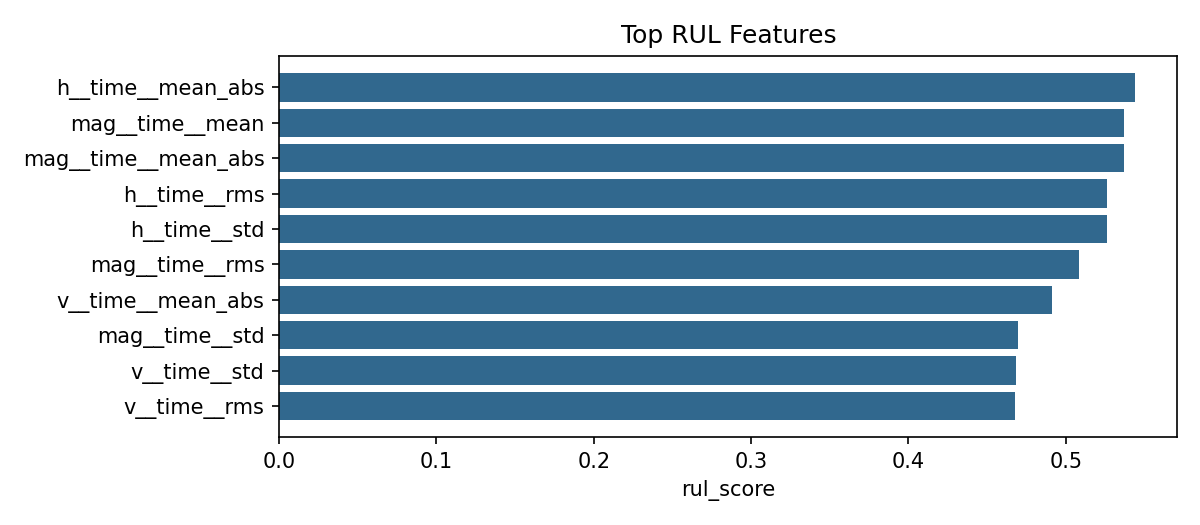
\includegraphics[width=0.92\textwidth]{phm2012/manual/rul_top_features.png}
\caption{PHM2012 official split 下 RUL 任务的 top features。}
\label{fig:phm2012_rul_top_features}
\end{figure}

图 \ref{fig:phm2012_rul_top_features} 显示 horizontal 和 magnitude amplitude 特征占据前列。

读图时应先看非 label-source 特征。

\feature{h__time__mean_abs} 是最重要的独立候选。

\feature{mag__time__mean} 和 \feature{mag__time__mean_abs} 提供 magnitude 方向的支持。

\feature{mag__time__rms} 若出现在前列，只能作为 Reference。

这张图支撑 PHM2012 RUL 的结论：以 horizontal amplitude 为第一候选，magnitude amplitude 为共同退化信号。

\subsection{Health State 特征分析}

PHM2012 Health State strongly favors horizontal-channel amplitude features。

\feature{h__time__mean_abs} 的 health score 为 0.944，rank 1。

它的 mutual information 为 0.486，Fisher score 为 0.789，ANOVA F 为 1979.4。

这三个指标共同说明，\feature{h__time__mean_abs} 对伪健康阶段有明显分离能力。

\feature{h__time__std} 和 \feature{h__time__rms} 分别 rank 2 和 rank 3。

它们的 boxplot 形态接近，说明 horizontal dispersion 和 energy 是同一退化现象的不同统计表达。

\feature{mag__time__mean} 和 \feature{mag__time__mean_abs} 是 B 级支持。

它们不如 horizontal top features 强，但仍有稳定分离能力。

\feature{mag__spectral__entropy} 进入 C 级。

它说明频谱复杂度在 PHM2012 Health State 中有辅助信号，但不是主线。

\begin{figure}[H]
\centering
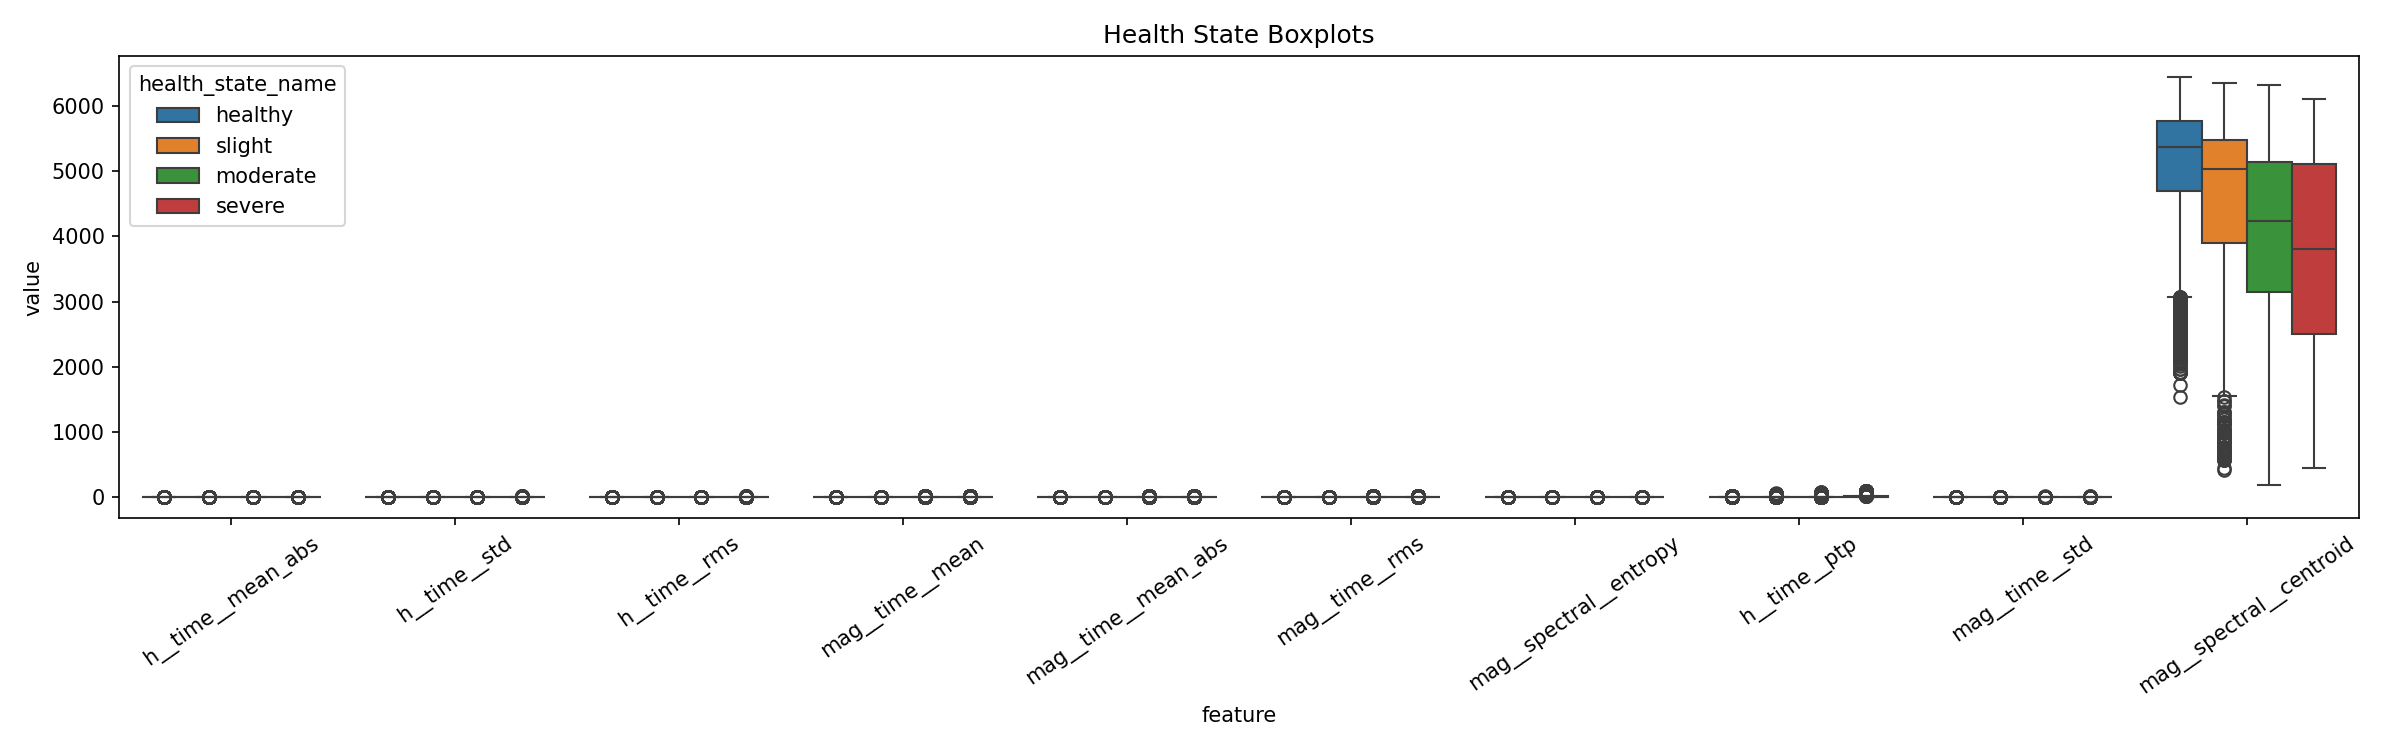
\includegraphics[width=0.92\textwidth]{phm2012/manual/health_state_boxplots.png}
\caption{PHM2012 official split 下 Health State 的箱线图。}
\label{fig:phm2012_health_boxplots}
\end{figure}

图 \ref{fig:phm2012_health_boxplots} 的重点是水平通道幅值类特征的状态分布。

如果健康阶段越严重，中位数和箱体整体上移，就说明该特征与退化阶段一致。

PHM2012 中，\feature{h__time__mean_abs}、\feature{h__time__std}、\feature{h__time__rms} 具有清晰的状态分离。

这和 XJTU-SY Step F 的 horizontal pattern 一致。

但 PHM2012 没有像 XJTU-SY 那样做跨工况 train=one-condition/test=another-condition 的压力测试。

所以最终写法应是：PHM2012 official split 支持 horizontal amplitude Health State；跨数据集共同主线仍是 amplitude family。

\subsection{Early Fault 特征分析}

PHM2012 Early Fault 同样由 amplitude family 主导。

\feature{h__time__mean_abs} rank 1，early fault score 为 0.994。

它的 AUC 为 0.836，Cohen's d 为 1.000，mean shift 为 0.220。

这说明 FPT 后水平平均绝对幅值明显上升。

\feature{mag__time__mean} 和 \feature{mag__time__mean_abs} 并列 rank 2。

它们的 AUC 为 0.824，Cohen's d 为 1.012，mean shift 为 0.317。

这说明 magnitude amplitude 对 FPT 前后分离同样有效。

\feature{h__time__std} 和 \feature{h__time__rms} 是 strong secondary。

它们捕捉的是水平通道离散度和能量增加。

这和早期故障中振动冲击/幅值扩大的物理直觉一致。

频域特征如 \feature{v__spectral__rms_frequency} 和 \feature{v__spectral__peak_frequency} 出现在 C 级。

它们有一定 pre/post FPT 分离能力，但不如 amplitude family 稳定。

\begin{figure}[H]
\centering
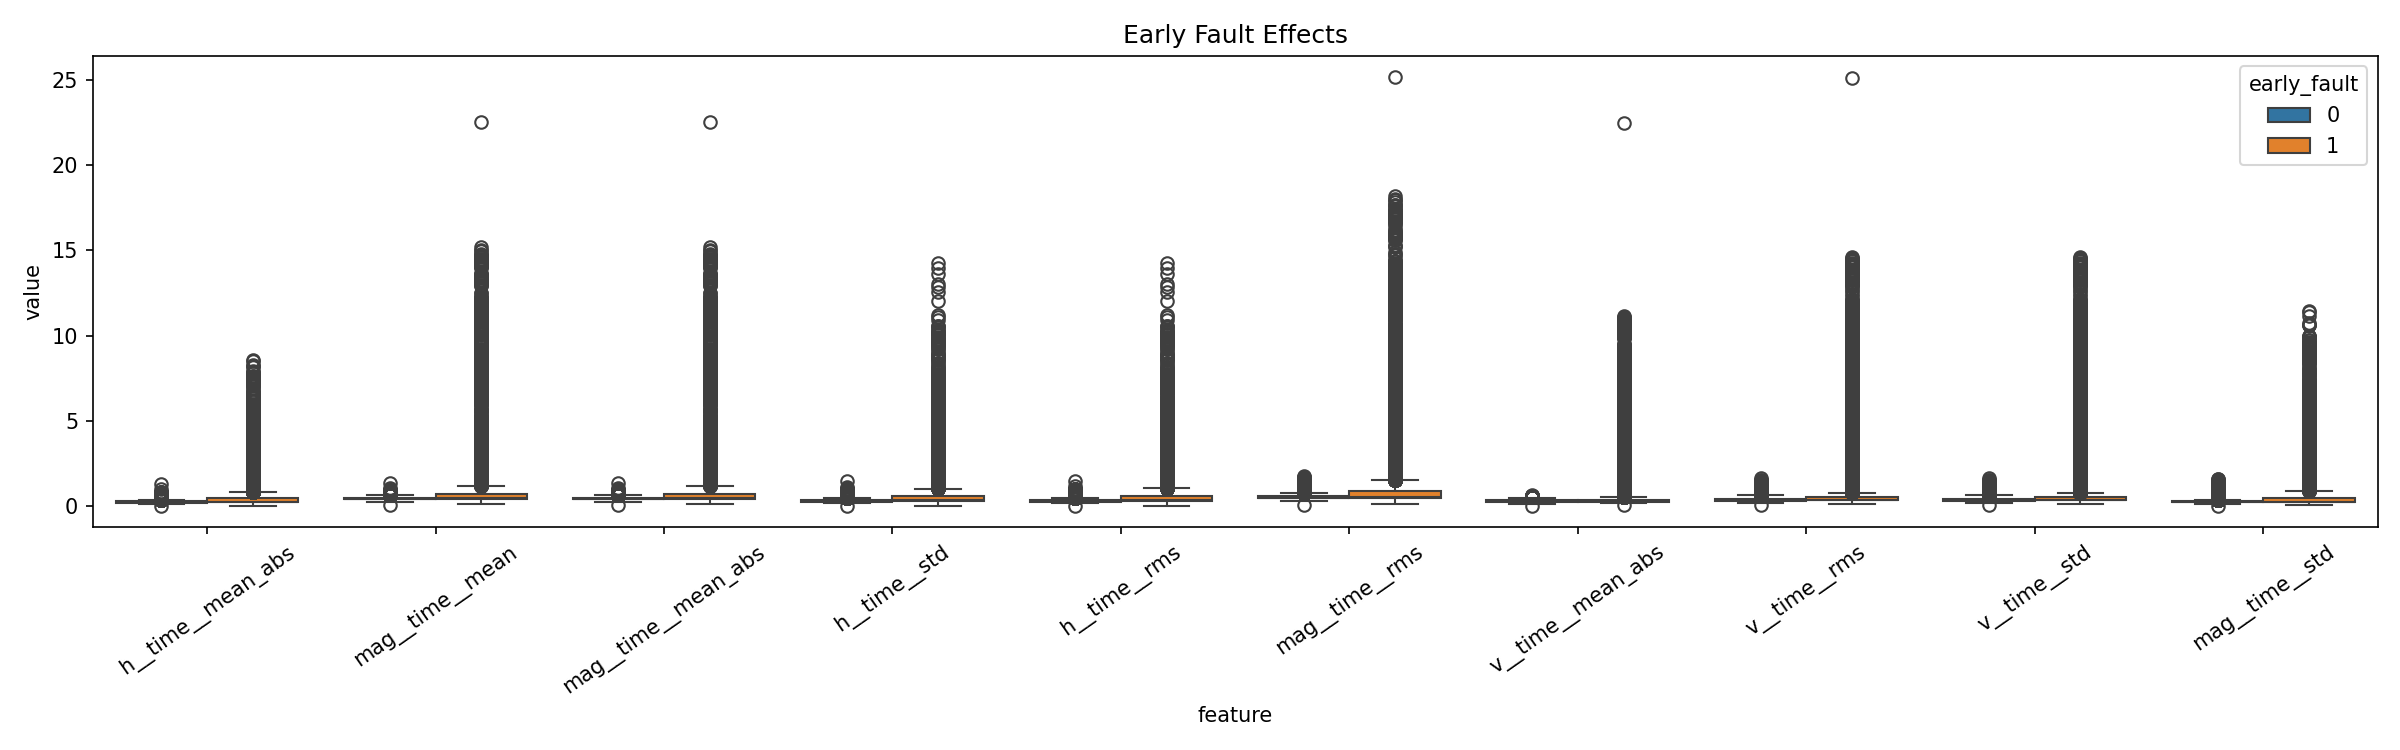
\includegraphics[width=0.92\textwidth]{phm2012/manual/early_fault_effects.png}
\caption{PHM2012 official split 下 Early Fault 的特征效应图。}
\label{fig:phm2012_early_fault_effects}
\end{figure}

图 \ref{fig:phm2012_early_fault_effects} 需要看 FPT 前后均值差和分布重叠。

PHM2012 中，horizontal/magnitude amplitude 特征在 FPT 后有明显上升。

这支撑把 \feature{h__time__mean_abs}、\feature{mag__time__mean}、\feature{mag__time__mean_abs} 放入 A 级。

同时，图也提醒我们 Early Fault 是 pseudo-label。

如果某个 Reference 特征强，只能说明它和 HI/FPT 规则一致。

非 label-source 的 horizontal/magnitude amplitude 特征才是独立候选。

\subsection{\config{manual_tsfresh_basic} 对照}

Step K 在 PHM2012 上成功运行 full-size \config{manual_tsfresh_basic}。

该 ranking 中有 44 个 ranked features，其中 20 个为 \feature{tsfresh__} 特征。

两个长度特征 \feature{tsfresh__h__length} 和 \feature{tsfresh__v__length} 因为常量被清理掉。

\begingroup
\scriptsize
\setlength{\tabcolsep}{3pt}
\renewcommand{\arraystretch}{1.18}
\begin{longtable}{@{}p{2.1cm}p{1.3cm}p{5.2cm}p{5.4cm}@{}}
\caption{PHM2012 manual\_tsfresh\_basic 对照}
\label{tab:phm2012_tsfresh_comparison}\\
\toprule
任务 & 数量 & 代表 tsfresh 特征 & 解释与决策 \\
\midrule
\endfirsthead
\toprule
任务 & 数量 & 代表 tsfresh 特征 & 解释与决策 \\
\midrule
\endhead
RUL & 5 & \feature{tsfresh__h__root_mean_square}; \feature{tsfresh__h__standard_deviation}; \feature{tsfresh__h__variance} & 重复 RMS/std/variance amplitude 信息；不改变主线。\\
Health State & 4 & \feature{tsfresh__h__standard_deviation}; \feature{tsfresh__h__root_mean_square}; \feature{tsfresh__h__maximum} & 确认 horizontal amplitude story；没有新增物理特征族。\\
Early Fault & 4 & \feature{tsfresh__h__standard_deviation}; \feature{tsfresh__v__standard_deviation}; \feature{tsfresh__v__root_mean_square} & 支持幅值/离散度 pre/post FPT 变化；保留为后续工程候选，不进入当前主线。\\
\bottomrule
\end{longtable}
\endgroup


tsfresh 对照的关键不是“是否进入 top10”，而是“进入 top10 的东西是否提供新信息”。

RUL 中进入 top10 的 tsfresh 特征包括：

\begin{itemize}[leftmargin=2em]
  \item \feature{tsfresh__h__root_mean_square}
  \item \feature{tsfresh__h__standard_deviation}
  \item \feature{tsfresh__h__variance}
\end{itemize}

这些分别对应手工 RMS、standard deviation 和 variance。

Health State 中 \feature{tsfresh__h__maximum} 和 \feature{tsfresh__h__absolute_maximum} 提供的是 horizontal amplitude extreme。

Early Fault 中 vertical tsfresh standard deviation/root mean square 与手工 vertical dispersion/RMS 重复。

因此 Step K 的结论是：PHM2012 tsfresh 成功运行，但其有效信息主要重复 amplitude/statistical family。

\begin{figure}[H]
\centering
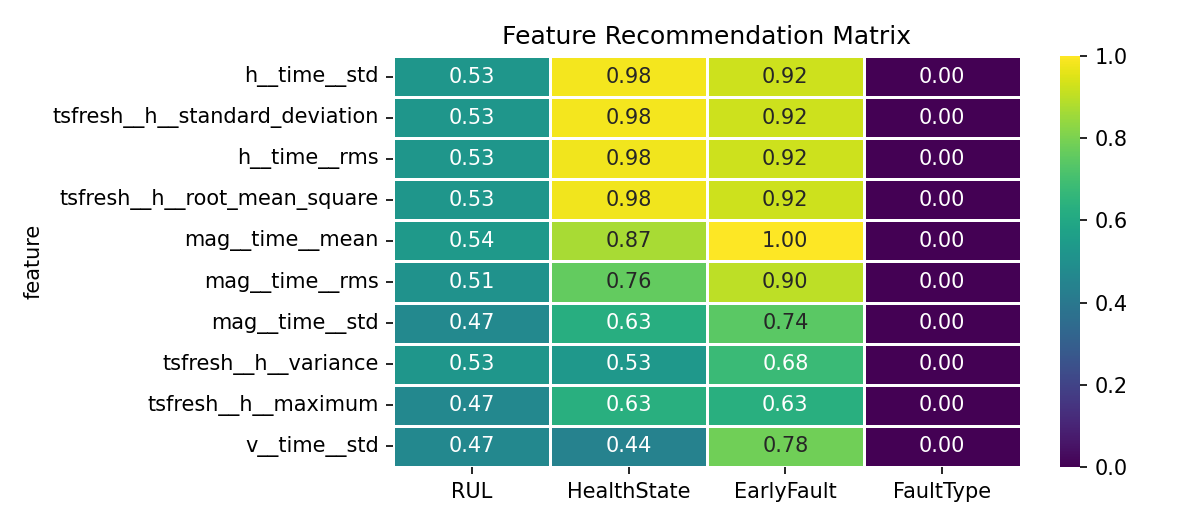
\includegraphics[width=0.92\textwidth]{phm2012/tsfresh/feature_recommendation_matrix.png}
\caption{PHM2012 \config{manual_tsfresh_basic} 的特征推荐矩阵。}
\label{fig:phm2012_tsfresh_recommendation_matrix}
\end{figure}

图 \ref{fig:phm2012_tsfresh_recommendation_matrix} 显示部分 \feature{tsfresh__} 特征进入 RUL、Health State 和 Early Fault 的推荐区域。

但是这些特征集中在 RMS、standard deviation、variance、maximum。

它们确认了 PHM2012 的 amplitude-dominant story。

它们没有提供足以替换 \config{manual_basic} 的新物理特征族。

\subsection{PHM2012 最终决策}

\begin{table}[htbp]
\centering
\caption{PHM2012 三任务推荐特征摘要}
\label{tab:phm2012_top_features}
\small
\begin{tabularx}{\textwidth}{lYYY}
\toprule
任务 & A 级 & B 级 & C 级或 Reference \\
\midrule
RUL & \feature{h__time__mean_abs}, \feature{mag__time__mean}, \feature{mag__time__mean_abs} & \feature{h__time__rms}, \feature{h__time__std}, \feature{v__time__mean_abs}, \feature{mag__time__std} & Reference: \feature{mag__time__rms} \\
Health State & \feature{h__time__mean_abs}, \feature{h__time__std}, \feature{h__time__rms} & \feature{mag__time__mean}, \feature{mag__time__mean_abs} & C: \feature{mag__spectral__entropy}; Reference: \feature{mag__time__rms} \\
Early Fault & \feature{h__time__mean_abs}, \feature{mag__time__mean}, \feature{mag__time__mean_abs} & \feature{h__time__std}, \feature{h__time__rms}, \feature{v__time__mean_abs}, \feature{v__time__std} & C: \feature{v__spectral__rms_frequency}, \feature{v__spectral__peak_frequency}; Reference: \feature{mag__time__rms} \\
\bottomrule
\end{tabularx}
\end{table}


PHM2012 的主线特征集仍为 \config{manual_basic}。

RUL 使用 \feature{h__time__mean_abs} 与 magnitude amplitude。

Health State 使用 horizontal amplitude family。

Early Fault 使用 horizontal/magnitude amplitude，并把 spectral frequency 作为 C 级 secondary。

\config{manual_tsfresh_basic} 可运行，但当前不作为主线。

后续如果要把 tsfresh 纳入 baseline，需要先证明它带来的不是 RMS/std/variance 的重复，而是对模型泛化或解释性有实际增益。

\section{跨数据集讨论}

\subsection{共同模式}

XJTU-SY 与 PHM2012 的共同结论是：振幅/能量类时域特征是最稳定的主线特征族。RUL、Health State 和 Early Fault 三个任务都能从 mean、mean absolute、RMS、standard deviation 等特征中获得强信号。

这种结果符合轴承退化的直观解释：随着损伤发展，振动幅值、能量和离散程度通常会增加。

\subsection{主要差异}

\begin{itemize}
  \item XJTU-SY 的 Early Fault 最工况敏感，不同工况下可能偏 spectral entropy、peak-to-peak 或 horizontal amplitude。
  \item PHM2012 更稳定地呈现 horizontal/magnitude amplitude dominant 模式。
  \item XJTU-SY full-size tsfresh blocked，而 PHM2012 tsfresh successful but redundant。
\end{itemize}

\subsection{tsfresh 的位置}

tsfresh 在本轮不进入主线。原因不是它一定无用，而是当前证据不足以替换 \config{manual_basic}：

\begin{itemize}
  \item XJTU-SY 不能在当前 backend 下完成 full-size 对照。
  \item PHM2012 虽能完成，但 top \feature{tsfresh__} 特征重复手工统计。
  \item 后续若要采用 tsfresh，需要单独的工程优化和更严格的增益评估。
\end{itemize}

\section{最终推荐特征}

\subsection{推荐表来源}

完整机器可读推荐表位于：

\begin{center}
\path{../summary/recommended_features.csv}
\end{center}

该表包含 dataset、analysis scope、task、feature、feature family、recommendation level、rank/score/plot evidence、label-source 标记、caveat 和 final decision。

LaTeX 中的 compact 表只摘取核心结论。

真正做 baseline planning 时，应以 CSV 为准。

\begingroup
\scriptsize
\setlength{\tabcolsep}{3pt}
\renewcommand{\arraystretch}{1.18}
\begin{longtable}{@{}p{1.7cm}p{1.9cm}p{4.2cm}p{2.3cm}p{4.8cm}@{}}
\caption{两个数据集上的最终推荐特征族}
\label{tab:final_recommended_features}\\
\toprule
数据集 & 任务 & A 级特征 & Reference & 说明 \\
\midrule
\endfirsthead
\toprule
数据集 & 任务 & A 级特征 & Reference & 说明 \\
\midrule
\endhead
XJTU-SY & RUL & \feature{mag__time__mean}, \feature{mag__time__mean_abs}, \feature{mag__time__std} & \feature{mag__time__rms} & 幅值和能量类时域特征在主划分、工况内和跨工况检查中都较稳定。\\
XJTU-SY & Health State & \feature{mag__time__mean}, \feature{mag__time__mean_abs}, \feature{mag__time__std} & \feature{mag__time__rms} & 主划分中水平通道较强，但跨工况检查中 magnitude 特征更稳。\\
XJTU-SY & Early Fault & \feature{mag__time__mean}, \feature{mag__time__mean_abs} & \feature{mag__time__rms} & 早期故障最工况敏感，horizontal 和 spectral 特征只作条件性辅助。\\
PHM2012 & RUL & \feature{h__time__mean_abs}, \feature{mag__time__mean}, \feature{mag__time__mean_abs} & \feature{mag__time__rms} & 水平通道与 magnitude 幅值特征主导。\\
PHM2012 & Health State & \feature{h__time__mean_abs}, \feature{h__time__std}, \feature{h__time__rms} & \feature{mag__time__rms} & 水平通道幅值类特征分离健康状态最强。\\
PHM2012 & Early Fault & \feature{h__time__mean_abs}, \feature{mag__time__mean}, \feature{mag__time__mean_abs} & \feature{mag__time__rms} & 幅值类特征主导，频域特征只作为 secondary 信号。\\
\bottomrule
\end{longtable}
\endgroup


\subsection{A/B/C/Reference 的使用边界}

A 级特征是主线候选。

它们通常同时满足：主划分排名靠前、稳定性检查支持、不是 label-source、物理解释清晰。

B 级特征是 secondary 候选。

它们可能与 A 级高度冗余，或者在某些 split 上略弱，但仍然能为模型提供稳定信号。

C 级特征是条件性候选。

它们适合做 ablation、诊断或工况敏感分析，不适合直接作为跨数据集主线。

Reference 特征主要是 \feature{mag__time__rms}。

它用于检查 HI/FPT 标签构造是否和振动能量一致。

它不用于证明 Health State 或 Early Fault 的独立可检测性。

\subsection{RUL 推荐说明}

RUL 的跨数据集共同推荐是 amplitude / energy-like features。

XJTU-SY 的 A 级是：

\begin{itemize}[leftmargin=2em]
  \item \feature{mag__time__mean}
  \item \feature{mag__time__mean_abs}
  \item \feature{mag__time__std}
\end{itemize}

PHM2012 的 A 级是：

\begin{itemize}[leftmargin=2em]
  \item \feature{h__time__mean_abs}
  \item \feature{mag__time__mean}
  \item \feature{mag__time__mean_abs}
\end{itemize}

这些特征的依据包括 RUL correlation、degradation score、curves 和稳定性检查。

RUL compact subset 可以选择非 label-source 的 magnitude/horizontal amplitude 特征。

\feature{mag__time__rms} 可以作为 reference ablation，但不应成为唯一主特征。

\subsection{Health State 推荐说明}

Health State 的共同模式也是 amplitude-driven。

XJTU-SY 最终更推荐 magnitude features，因为 cross-condition 后它们更稳。

PHM2012 更推荐 horizontal features，因为 official split 中 \feature{h__time__mean_abs}、\feature{h__time__std}、\feature{h__time__rms} 的 boxplot 和统计指标都很强。

Health State 的 baseline 设计应同时考虑两个版本：

\begin{itemize}[leftmargin=2em]
  \item dataset-specific compact set：XJTU 用 magnitude，PHM 用 horizontal；
  \item unified compact set：magnitude + horizontal amplitude 共同输入，让模型自己学习权重。
\end{itemize}

如果包含 \feature{mag__time__rms}，需要在报告里标明它是 Reference。

\subsection{Early Fault 推荐说明}

Early Fault 不能只看主划分 top rank。

PHM2012 中 amplitude features 较稳定。

XJTU-SY 中 Early Fault 工况敏感。

因此推荐策略是：

\begin{itemize}[leftmargin=2em]
  \item PHM2012：以 \feature{h__time__mean_abs}、\feature{mag__time__mean}、\feature{mag__time__mean_abs} 为 A 级；
  \item XJTU-SY：以 \feature{mag__time__mean}、\feature{mag__time__mean_abs} 为 A 级；
  \item XJTU-SY：把 horizontal amplitude、spectral entropy、peak-to-peak/shock-like 特征作为 C 级 ablation；
  \item 两个数据集：\feature{mag__time__rms} 只作 Reference。
\end{itemize}

Early Fault baseline 的报告必须包含 caveat。

特别是 XJTU-SY，如果某个模型在主 split 上表现好，还需要 condition-wise 或 cross-condition 结果支撑。

\subsection{Compact Baseline Subset}

\begin{table}[htbp]
\centering
\caption{下游 baseline 的 compact feature subset 建议}
\label{tab:compact_baseline_suggestions}
\scriptsize
\begin{tabularx}{\textwidth}{lYY}
\toprule
用途 & 建议特征 & 使用边界 \\
\midrule
Full manual set & \config{manual_basic} 全部 45 个特征 & 作为默认 baseline 输入，需 train-only scaling。\\
Compact RUL & \feature{mag__time__mean}, \feature{mag__time__mean_abs}, \feature{mag__time__std}, \feature{h__time__mean_abs}, \feature{h__time__std}, \feature{v__time__std} & 排除或单独报告 \feature{mag__time__rms}。\\
Compact Health & XJTU: magnitude mean/std；PHM: \feature{h__time__mean_abs}, \feature{h__time__std}, \feature{h__time__rms} & 数据集感知通道选择，避免把 PHM horizontal 结论直接迁移到 XJTU cross-condition。\\
Compact Early Fault & \feature{mag__time__mean}, \feature{mag__time__mean_abs}, \feature{mag__time__std}, \feature{h__time__mean_abs}, \feature{v__time__std} & XJTU 加 C 级 spectral/shock 特征做 ablation；PHM 主线仍用 amplitude。\\
Reference ablation & \feature{mag__time__rms} & 只用于 sanity/reference 或单独消融，不作为独立发现。\\
\bottomrule
\end{tabularx}
\end{table}


Full feature set 是 \config{manual_basic} 全 45 个特征。

它适合作为默认输入。

Compact subset 的作用是提高解释性和减少冗余。

RUL compact subset 应优先保留 non-label-source amplitude features。

Health compact subset 应按数据集选择 channel。

Early Fault compact subset 应保留 A/B 主线，并把 C 级特征用于 ablation。

\subsection{冗余与消融}

很多 top features 是同一物理现象的重复表达。

例如：

\begin{itemize}[leftmargin=2em]
  \item \feature{mag__time__mean} 与 \feature{mag__time__mean_abs} 在当前 magnitude 构造下几乎等价；
  \item \feature{h__time__rms} 与 \feature{h__time__std} 高度相关；
  \item tsfresh 的 RMS/std/variance 与 manual features 重复；
  \item \feature{mag__time__rms} 和其他 magnitude amplitude 特征相关，但它同时是 label-source。
\end{itemize}

因此，baseline 不应只报告“全特征最好”。

更有解释价值的做法是报告：

\begin{itemize}[leftmargin=2em]
  \item full \config{manual_basic}；
  \item compact non-label-source subset；
  \item compact + Reference；
  \item dataset-specific C-level ablation。
\end{itemize}

这样才能区分“真实可泛化特征”与“标签构造参考特征”。

\section{局限性}

本报告存在以下局限性：

\begin{enumerate}
  \item Health State 和 Early Fault 是由 HI/FPT 构造的 pseudo labels，不是人工标注的真实故障阶段。
  \item \feature{mag__time__rms} 是实际 label-source feature，因此只能作为 Reference，不能作为独立证据过度解释。
  \item XJTU-SY Early Fault 显著工况敏感，需要在后续 baseline 中进行工况分层或跨工况验证。
  \item PHM2012 official split 中部分 amplitude 特征在 val/test 上方差更大，模型评估需要谨慎解释。
  \item XJTU-SY full-size tsfresh 在当前 backend 下存在内存问题，尚未完成公平对照。
  \item 当前未设计 BPFO、BPFI、BSF、FTF 等轴承机理频率特征。
  \item 本报告不包含模型训练、baseline recipes、checkpoint 或 prediction 结果。
\end{enumerate}

这些局限性不会否定 \config{manual_basic} 的主线价值，但会影响后续 baseline 的实验设计和解释边界。

\section{结论}

本轮特征分析已经完成两个数据集、三个任务和两个特征集方向的收敛。

最终决策：

\begin{center}
\config{manual_basic} 是当前 downstream baseline 的主特征集。
\end{center}

任务级结论：

\begin{itemize}
  \item RUL：优先使用振幅/能量类时域特征。
  \item Health State：优先使用幅值类特征，XJTU-SY 需考虑 cross-condition 稳定性，PHM2012 更偏 horizontal 通道。
  \item Early Fault：PHM2012 仍由幅值类特征主导；XJTU-SY 需要明确工况敏感 caveat。
\end{itemize}

\feature{mag__time__rms} 保留为 label-source reference，不作为独立发现证据。

下一步应进入 baseline planning。后续实验应基于 \config{manual_basic} 和最终推荐表：

\begin{center}
\path{../summary/recommended_features.csv}
\end{center}

然后分别设计 RUL 回归、Health State 分类和 Early Fault Detection 的可复现实验。


\bibliographystyle{plain}
\bibliography{references}

\end{document}
